% Section 6: Ensembles, Random Forest, and XGBoost (Slides 40-47)

% Slide 40: How to Prevent Overfitting 1: More Training Data
\begin{frame}{پیشگیری از بیش‌برازش: افزایش حجم داده‌های آموزش}{\lr{Prevention 1: Use More Training Data}}
  \begin{center}
    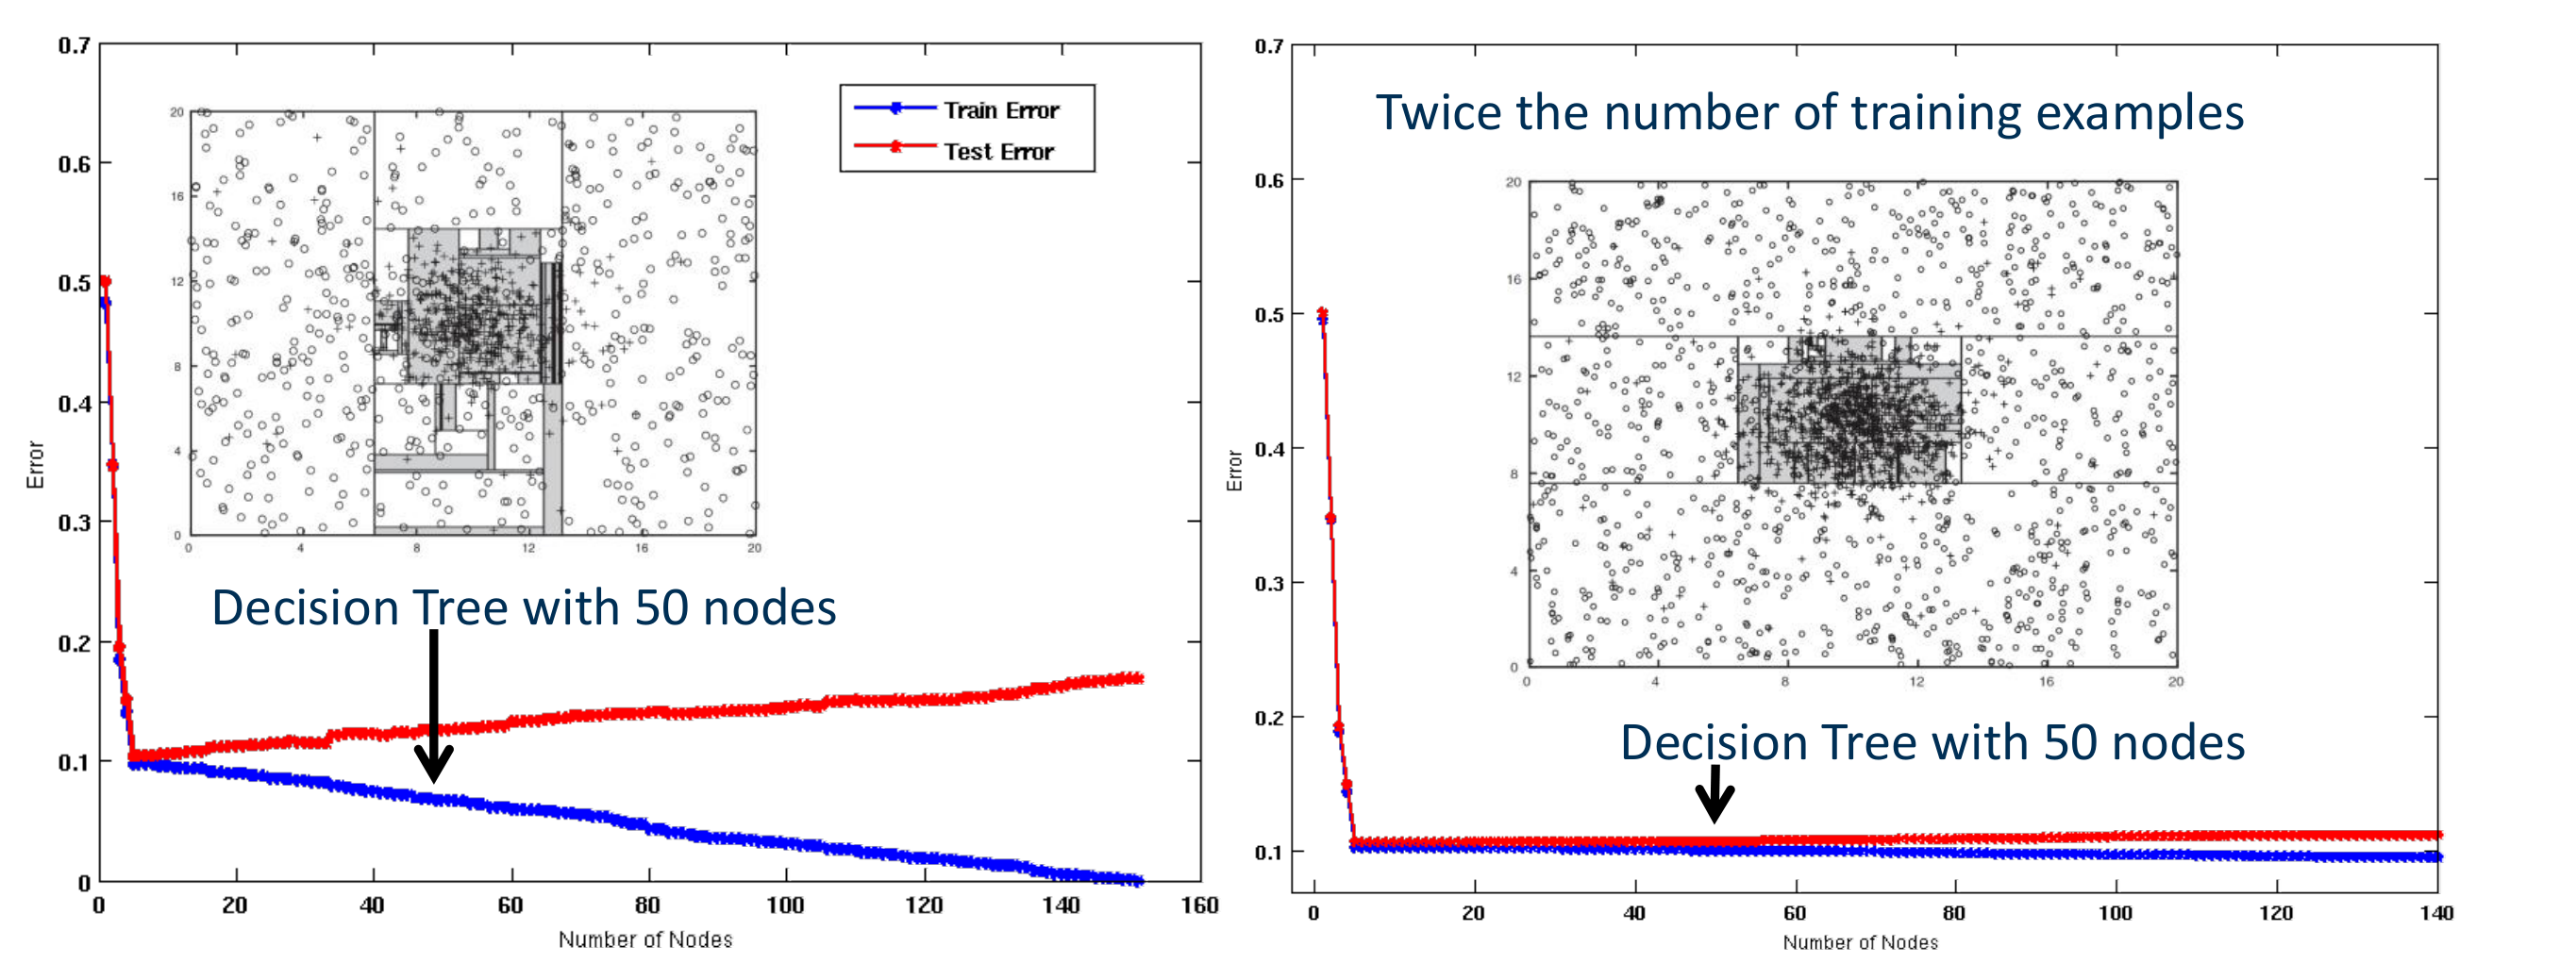
\includegraphics[width=0.95\textwidth,height=3.4cm,keepaspectratio]{images/slide40_two_error_curves.png}
  \end{center}
  \vspace{0.1cm}
  \begin{itemize}
    \setlength{\itemsep}{5pt}
    \item در صورت ناکافی بودن داده‌های آموزش، با افزایش عمق درخت، خطای آزمون به سرعت اوج می‌گیرد.
    \item افزایش حجم داده‌های آموزش، فاصله میان خطای آموزش و آزمون را به حداقل رسانده و از بیش‌برازش جلوگیری می‌کند.
  \end{itemize}
\end{frame}

% Slide 41: How to Prevent Overfitting 2: Pre-Pruning
\begin{frame}{پیشگیری از بیش‌برازش: پیش‌هرس درخت}{\lr{Prevention 2: Pre-Pruning}}
  \begin{itemize}
    \setlength{\itemsep}{7pt}
    \item \textbf{ایده اصلی:} متوقف کردن رشد درخت پیش از آنکه بیش از حد عمیق و منشعب شود (تیغ اوکام).
    \item \textbf{شرایط توقف عادی (بدون هرس):}
    \begin{itemize}
      \item تمام نمونه‌های موجود در گره متعلق به یک کلاس باشند.
      \item مقادیر تمام ویژگی‌ها برای نمونه‌های باقیمانده یکسان باشد.
    \end{itemize}
    \item \textbf{معیارهای پیش‌هرس زودهنگام:} \lr{(Pre-Pruning)}
    \begin{itemize}
      \item تعیین سقف برای بیشینه عمق درخت (\codeinline{max\_depth})
      \item حداقل نمونه لازم برای انشعاب گره (\codeinline{min\_samples\_split})
      \item حداقل نمونه لازم در هر برگ (\codeinline{min\_samples\_leaf})
      \item توقف در صورت عدم دستیابی به حداقل بهبود ناخالصی (\codeinline{min\_impurity\_decrease})
    \end{itemize}
  \end{itemize}
\end{frame}

% Slide 42: How to Prevent Overfitting 3: Ensembles
\begin{frame}{پیشگیری از بیش‌برازش: روش‌های جمعی}{\lr{Prevention 3: Ensembles}}
  \begin{itemize}\setlength{\itemsep}{2pt}
    \item \textbf{یادگیری جمعی (\lr{Ensemble}):} آموزش چندین مدل پایه
    \item \textbf{رأی‌گیری جمعی (\lr{Voting}):} رأی‌گیری میان مدل‌ها برای تصمیم نهایی
  \end{itemize}
  \begin{center}
    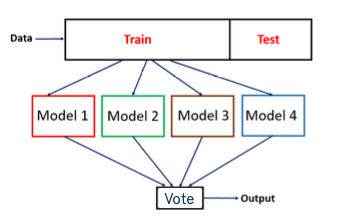
\includegraphics[width=0.62\textwidth,height=2.3cm,keepaspectratio]{images/slide42_ensemble_diagram_clean.png}
  \end{center}
  \begin{itemize}\setlength{\itemsep}{2pt}
    \item \textbf{ایده خرد جمعی (\lr{Wisdom of the Crowds}) در دسته‌بندی:}
    \begin{itemize}\setlength{\itemsep}{1pt}
      \item یک کلاسیفایر منفرد ممکن است بر یک جنبه متمرکز شده یا به نویز حساس باشد.
      \item مدل‌های متنوع جنبه‌های مختلف را فرا گرفته و خطاهای تصادفی یکدیگر را خنثی می‌کنند.
    \end{itemize}
  \end{itemize}
\end{frame}

% Slide 43: Algorithms to Learn Tree Ensembles
\begin{frame}{الگوریتم‌های یادگیری جمعی درخت‌ها}{\lr{Tree Ensemble Algorithms}}
  \begin{itemize}
    \setlength{\itemsep}{10pt}
    \item \textbf{جنگل تصادفی (\lr{Random Forest} -- برایمن، ۱۹۹۷)}
    \begin{itemize}
      \item ترکیب درخت‌های مستقل با استفاده از بگینگ و انتخاب تصادفی ویژگی‌ها
      \item \codeinline{sklearn.ensemble.RandomForestClassifier}
    \end{itemize}
    \item \textbf{افزایش گرادیانی درخت‌ها (\lr{Gradient Tree Boosting} -- فریدمن، ۱۹۹۹)}
    \begin{itemize}
      \item بهینه‌سازی ترتیبی با تمرکز بر تصحیح خطای مراحل پیشین
      \item \codeinline{sklearn.ensemble.GradientBoostingClassifier}
    \end{itemize}
    \item \textbf{بوستینگ منظم‌شده و بسیار مقیاس‌پذیر:} \lr{(XGBoost)}
    \begin{itemize}
      \item سیستم فوق‌سریع و توزیع‌شده با کنترل دقیق پیچیدگی مدل (\lr{Regularization})
    \end{itemize}
  \end{itemize}
\end{frame}

% Slide 44: Random Forest
\begin{frame}{جنگل تصادفی}{\lr{Random Forest}}
  \begin{itemize}
    \setlength{\itemsep}{7pt}
    \item \textbf{مفهوم:} مجموعه‌ای متشکل از صدها درخت تصمیم مستقل که طبقه‌بندی نهایی را با رأی اکثریت انجام می‌دهند.
    \item \textbf{ایجاد استقلال و تنوع میان درخت‌ها با دو سازوکار تصادفی:}
    \begin{enumerate}
      \setlength{\itemsep}{3pt}
      \item \textbf{بگینگ داده‌ها:} \lr{(Data Bagging)} هر درخت بر روی یک نمونه‌گیری تصادفی همراه با جایگذاری (\lr{Bootstrap}) آموزش می‌بیند.
      \item \textbf{انتخاب تصادفی ویژگی‌ها:} \lr{(Feature Subsampling)} در هر گره، تنها زیرمجموعه تصادفی کوچکی از ویژگی‌ها (معمولاً $\sqrt{p}$) آزمون می‌شود.
    \end{enumerate}
  \end{itemize}
  \vspace{0.15cm}
  \begin{center}
    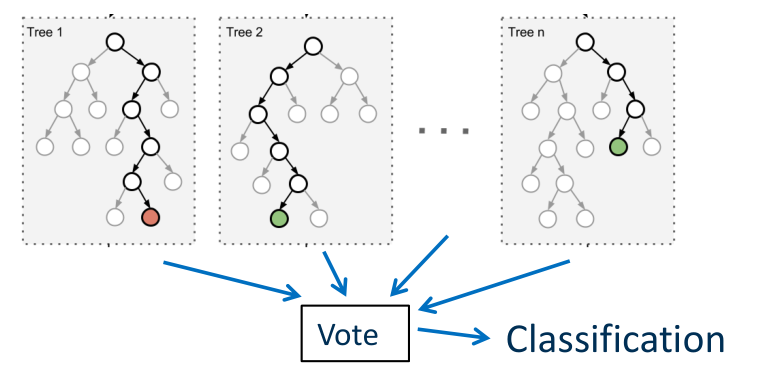
\includegraphics[width=0.75\textwidth,height=2.7cm,keepaspectratio]{images/slide44_random_forest_clean.png}
  \end{center}
\end{frame}

% Slide 45: Random Forest in Python
\begin{frame}{جنگل تصادفی در پایتون}{\lr{Random Forest in Python}}
  \begin{itemize}
    \setlength{\itemsep}{6pt}
    \item جنگل‌های تصادفی به دلیل کاهش چشمگیر واریانس، معمولاً عملکردی به مراتب برتر از تک‌درخت ارائه می‌دهند.
    \item پیاده‌سازی در کتابخانه \codeinline{scikit-learn}:
  \end{itemize}
  \vspace{0.15cm}
  \begin{latin}
  \begin{center}
    \fcolorbox{codeborder}{codebg}{
      \begin{minipage}{0.92\textwidth}
        \ttfamily\small
        \textbf{from} sklearn.ensemble \textbf{import} RandomForestClassifier\\[6pt]
        \textcolor{gray}{\# Train classifier}\\
        forest\_estimator = RandomForestClassifier(n\_estimators=100, criterion=\textcolor{teal}{'gini'}, max\_depth=None)\\
        forest\_estimator.fit(preprocessed\_training\_data, training\_labels)\\[6pt]
        \textcolor{gray}{\# Use classifier to predict labels}\\
        prediction = forest\_estimator.predict(preprocessed\_unseen\_data)
      \end{minipage}
    }
  \end{center}
  \end{latin}
\end{frame}

% Slide 46: XGBoost Objective
\begin{frame}{الگوریتم \lr{XGBoost} -- تابع هدف منظم‌شده}{\lr{eXtreme Gradient Boosting}}
  \begin{itemize}
    \item \textbf{سیستم مقیاس‌پذیر برای یادگیری مجموعه‌ای از درخت‌ها:}
  \end{itemize}
  \vspace{0.1cm}
  \begin{center}
    \fcolorbox{mannheimblue}{codebg}{
      \Large $\displaystyle \text{Obj}(\Theta) = L(\Theta) + \Omega(\Theta)$
    }
  \end{center}
  \vspace{0.15cm}
  \begin{columns}[T]
    \begin{column}{0.48\textwidth}
      \begin{block}{تابع زیان آموزش: $L(\Theta)$}
        \begin{itemize}
          \setlength{\itemsep}{3pt}
          \item کیفیت پیش‌بینی و برازش بر داده‌ها
          \item کمینه‌سازی آن منجر به مدل‌های پیش‌بینانه قوی می‌شود.
        \end{itemize}
      \end{block}
    \end{column}
    \begin{column}{0.48\textwidth}
      \begin{block}{جمله منظم‌سازی: $\Omega(\Theta)$}
        \begin{itemize}
          \setlength{\itemsep}{3pt}
          \item جریمه پیچیدگی ساختار درخت‌ها
          \item کمینه‌سازی آن منجر به مدل‌های ساده و پایدار می‌شود.
        \end{itemize}
      \end{block}
    \end{column}
  \end{columns}
  \vspace{0.1cm}
  \begin{itemize}
    \item \textbf{بهینه‌سازی‌های سیستمی:} محاسبات خارج از حافظه (\lr{Out-of-core})، موازی‌سازی و بهینه‌سازی حافظه پنهان (\lr{Cache-aware}).
  \end{itemize}
\end{frame}

% Slide 47: XGBoost Additive Training
\begin{frame}{الگوریتم \lr{XGBoost} -- یادگیری افزایشی و منظم‌سازی}{\lr{Additive Training and Regularization}}
  \begin{columns}[T]
    \begin{column}{0.56\textwidth}
      \begin{itemize}
        \setlength{\itemsep}{5pt}
        \item \textbf{یادگیری افزایشی:} \lr{(Additive Training)}
        \[
          \hat{y}_i^{(t)} = \hat{y}_i^{(t-1)} + f_t(x_i)
        \]
        در هر مرحله یک درخت جدید برای تصحیح خطای باقیمانده اضافه می‌شود.
        \item \textbf{تعریف پیچیدگی درخت تصمیم:}
        \[
          \Omega(f) = \gamma T + \frac{1}{2}\lambda \sum_{j=1}^T w_j^2
        \]
        \begin{itemize}
          \item $T$: تعداد گره‌های برگ درخت
          \item $w_j$: امتیاز (وزن) هر گره برگ
        \end{itemize}
      \end{itemize}
    \end{column}
    \begin{column}{0.42\textwidth}
      \begin{center}
        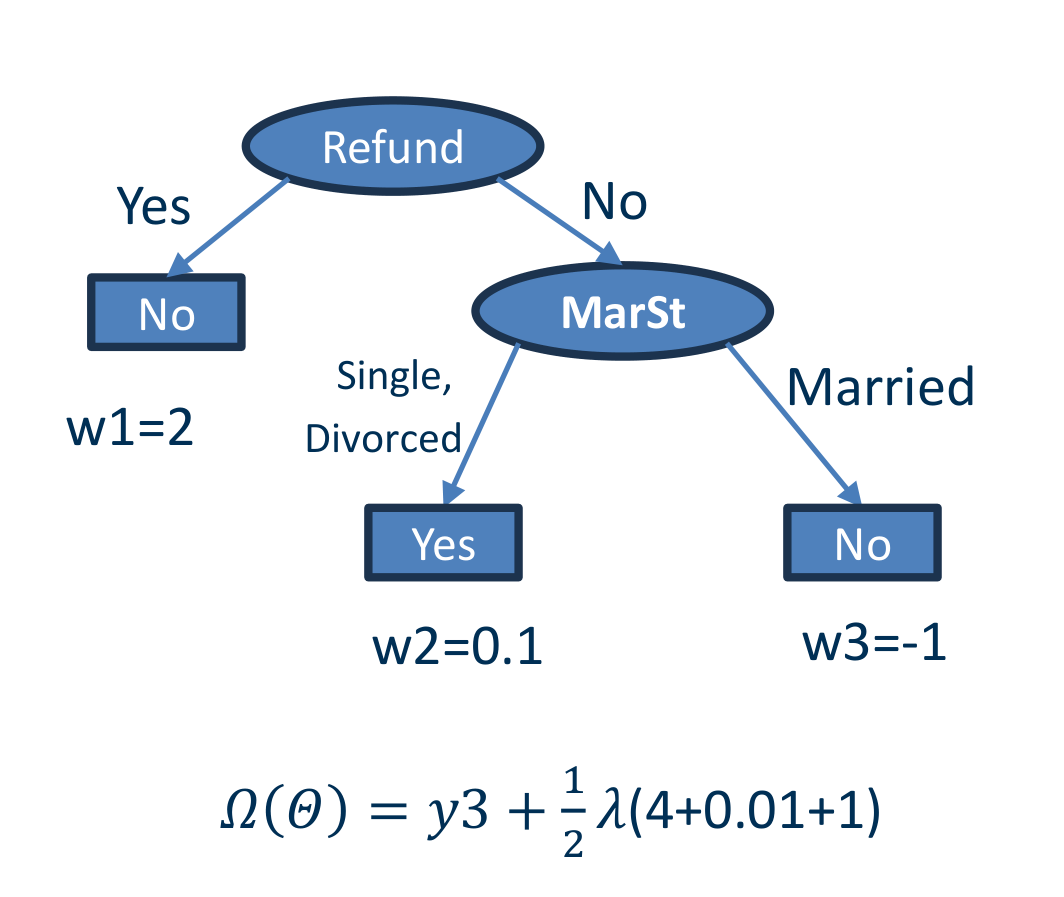
\includegraphics[width=\textwidth,height=3.4cm,keepaspectratio]{images/slide47_xgboost_tree_weights.png}\\[0.1cm]
        {\footnotesize $\Omega(\Theta) = \gamma \cdot 3 + \frac{1}{2}\lambda(4 + 0.01 + 1)$}
      \end{center}
    \end{column}
  \end{columns}
\end{frame}
